\section{Finding 18 - Hard Coded Credentials}

%center under chapter title a one row table with 6 coloumns and no borders
\vspace*{-0,3cm}
\begin{center}
    \begin{tabular}{c c c c}
        \textbf{Classification:} & Information Disclosure & \textbf{Severity:} & \textbf{\textcolor{orange}{Medium}}  
        \end{tabular}
\end{center}
After decrypting the ”container.img” on the \ac{DUT} a file callled ”crypofs\_init” can be found which contains hard coded credentials.
\subsection*{Finding Impact}
These credentials could be useful to gain access to the ”dhbw.johannes-bauer.com” system. 

\subsection*{Finding Details}
The ”cryptofs\_init” file looks like this:
%image
\begin{figure}[H]
    \centering
    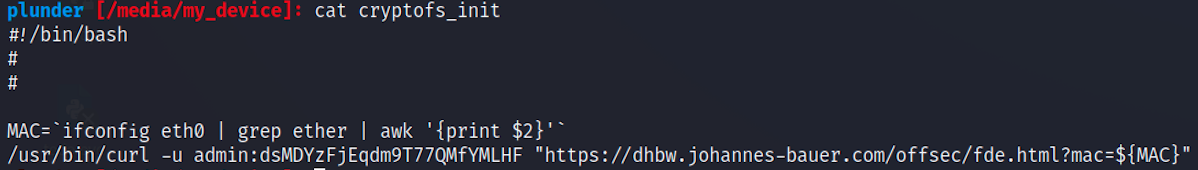
\includegraphics[width=1\textwidth]{img/Bildschirm­foto 2023-03-19 um 20.55.24.png}
    \label{fig:fin18}
\end{figure}
This script sends the \ac{DUT}s MAC address appended to the url ”dhbw.johannes-bauer.com/offsec”.
This could also be connected to the finding 16 beacause in both findings the MAC address is send to the same url.
\subsection*{Evaluation of Results}
\begin{center}
    \begin{tabular}{cccc}
    \textbf{Effort to Fix:} & &\ \textbf{\textcolor{orange}{Medium}}\
    \end{tabular}
\end{center}
Credentials never should be hardcoded in a script.